
\documentclass{beamer}
\usepackage[utf8x]{inputenc}

\usetheme{default}
\usepackage{setspace}
\usepackage{hyperref}

\usepackage{listings}
\definecolor{keywords}{RGB}{180,180,0}
\definecolor{comments}{RGB}{60,179,113}
% \definecolor{red}{RGB}{255,0,0}
\definecolor{darkgreen}{RGB}{0,127,0}
\lstset{
  language=Python,
  frame=lines,
  keywordstyle=\color{keywords},
  commentstyle=\color{comments}\emph,
  stringstyle=\ttfamily\color{darkgreen},
  emph={Soap11,XmlDocument,HtmlMicroFormat},emphstyle=\color{red}\textbf
}

\title{A Quick Look At Spyne}
\author{Burak Arslan \\ \small burak at arskom \small{dot} com \small{dot} tr}
\usepackage{wasysym}

\hypersetup{
   colorlinks,
   citecolor=blue,
   filecolor=blue,
   linkcolor=blue,
   urlcolor=blue,
   breaklinks=true
}

\setbeamertemplate{footline}{\hfill\scriptsize{\insertframenumber}\hspace*{.5cm}\vspace*{.5cm}}
\setbeamertemplate{navigation symbols}{}

\begin{document}

\begin{frame}
  \maketitle
\end{frame}

\begin{frame}
  \frametitle{What is Spyne?}

  \LARGE
  \begin{center}

    Spyne makes it convenient to

    \bigskip

    expose your services using multiple

    \bigskip

    protocols and/or transports.

  \end{center}

\end{frame}


% \begin{frame}
% \LARGE
% \begin{center}
%
%   Which seems to be especially important
%
%   \bigskip
%
%   for applications with multiple types of clients
%
%   \large
%
%   \bigskip
%
%   (Native apps, browsers, etc.)
%
% \end{center}
%
% \end{frame}


\begin{frame}
  \frametitle{What is Spyne?}

  \LARGE
  \begin{center}

    It also forces you to have a well-defined api.

%     \bigskip
%
%     \pause
%
%     Because static typing works wonders
%
%     \bigskip
%
%     when your input comes from untrusted sources

  \end{center}

\end{frame}


\begin{frame}
\Huge
\begin{center}

  How?

\end{center}

\end{frame}

\begin{frame}[fragile]
  \LARGE
\begin{center}

  Here's a simple function:

  \bigskip

  \bigskip

  \large

  \begin{lstlisting}
  from datetime import datetime

  def get_utc_time():
      return datetime.utcnow()
  \end{lstlisting}

\end{center}
\end{frame}

\begin{frame}
  \LARGE

  Now, to make this function remotely callable;

  \bigskip

\pause

  \color{red} \textbf{1)} \color{black}


    \begin{center}
      We wrap it in a \texttt{Service} subclass:
    \end{center}

\end{frame}

\begin{frame}[fragile]
\begin{uncoverenv}<2->
  \begin{lstlisting}[frame=none]
from spyne.model.primitive import DateTime
from spyne.decorator import srpc
from spyne.service import Service
  \end{lstlisting}
\end{uncoverenv}
\begin{uncoverenv}<3->
  \begin{lstlisting}[frame=none]
class DateTimeService(Service):
  \end{lstlisting}
  \vspace{-13pt}
\end{uncoverenv}
\begin{uncoverenv}<4->
  \begin{lstlisting}[frame=none]
    @srpc(_returns=DateTime)
  \end{lstlisting}
  \vspace{-13pt}
\end{uncoverenv}
\begin{uncoverenv}<1->
  \begin{lstlisting}[frame=none]
    def get_utc_time():
        return datetime.utcnow()
  \end{lstlisting}
\end{uncoverenv}
\end{frame}

\begin{frame}
  \LARGE

  \color{red} \textbf{2)} \color{black}

  \begin{center}
    Now, we have to wrap the service definition

    \bigskip

    in an \texttt{Application} definition.

  \end{center}

\end{frame}

\begin{frame}[fragile]
\begin{uncoverenv}<2->
  \vspace{-13pt}
  \begin{lstlisting}[frame=none]
from spyne.application import Application
from spyne.protocol.http import HttpRpc
  \end{lstlisting}
\end{uncoverenv}
\begin{uncoverenv}<2->
  \begin{lstlisting}[frame=none]
httprpc = Application(
  \end{lstlisting}
\end{uncoverenv}
\begin{uncoverenv}<1->
  \vspace{-13pt}
  \begin{lstlisting}[frame=none]
        [DateTimeService],
  \end{lstlisting}
\end{uncoverenv}
\begin{uncoverenv}<3->
  \vspace{-13pt}
  \begin{lstlisting}[frame=none]
        tns='spyne.examples.multiprot',
  \end{lstlisting}
\end{uncoverenv}
\begin{uncoverenv}<4->
  \vspace{-13pt}
  \begin{lstlisting}[frame=none]
        in_protocol=HttpRpc(),
        out_protocol=HttpRpc()
    )
  \end{lstlisting}
\end{uncoverenv}
\end{frame}

\begin{frame}
  \LARGE
  \color{red} \textbf{3)} \color{black}

  \begin{center}
    Finally, we wrap the application in

    \bigskip

    a transport.

  \end{center}

\end{frame}

\begin{frame}[fragile]
 \begin{lstlisting}
from spyne.server.wsgi import WsgiApplication

application = WsgiApplication(httprpc)
 \end{lstlisting}

  \begin{center}
    This is now a regular WSGI Application that

    \bigskip

    we can pass to WSGI-compliant servers like

    \bigskip

    CherryPy, mod\_wsgi, Twisted, etc.
  \end{center}
  \pause
  \begin{lstlisting}[language=sh]
$ curl http://localhost:9910/get_utc_time
2012-03-09T17:38:11.997784
  \end{lstlisting}
\end{frame}

\begin{frame}
  \LARGE
  \begin{center}
    Now, what if we wanted to expose this

    \bigskip

    function using another protocol?
  \end{center}
\end{frame}

\begin{frame}[fragile]
  \frametitle{For example: SOAP}

  \begin{lstlisting}
from spyne.application import Application
from spyne.protocol.http import HttpRpc
from spyne.protocol.soap import Soap11

soap = Application([DateTimeService],
        tns='spyne.examples.multiprot',
        in_protocol=HttpRpc(),
        out_protocol=Soap11()
    )
  \end{lstlisting}
\end{frame}

\begin{frame}[fragile]
  \frametitle{For example: SOAP}

  \begin{lstlisting}[language=sh,frame=topline]
$ curl http://localhost:9910/get_utc_time \
                              | tidy -xml -indent
  \end{lstlisting}
  \tiny
  \begin{lstlisting}[language=xml,frame=bottomline]
  <?xml version='1.0' encoding='utf-8'?>
  <senv:Envelope xmlns:wsa="http://schemas.xmlsoap.org/ws/2003/03/addressing"
  xmlns:tns="spyne.examples.multiple_protocols"
  xmlns:plink="http://schemas.xmlsoap.org/ws/2003/05/partner-link/"
  xmlns:xop="http://www.w3.org/2004/08/xop/include"
  xmlns:senc="http://schemas.xmlsoap.org/soap/encoding/"
  xmlns:s12env="http://www.w3.org/2003/05/soap-envelope"
  xmlns:s12enc="http://www.w3.org/2003/05/soap-encoding"
  xmlns:xs="http://www.w3.org/2001/XMLSchema"
  xmlns:wsdl="http://schemas.xmlsoap.org/wsdl/"
  xmlns:xsi="http://www.w3.org/2001/XMLSchema-instance"
  xmlns:senv="http://schemas.xmlsoap.org/soap/envelope/"
  xmlns:soap="http://schemas.xmlsoap.org/wsdl/soap/">
    <senv:Body>
      <tns:get_utc_timeResponse>
        <tns:get_utc_timeResult>
          2012-03-06T17:43:30.894466
        </tns:get_utc_timeResult>
      </tns:get_utc_timeResponse>
    </senv:Body>
  </senv:Envelope>
  \end{lstlisting}
\end{frame}

\begin{frame}[fragile]
  \frametitle{Or, just XML:}

  \begin{lstlisting}
from spyne.application import Application
from spyne.protocol.http import HttpRpc
from spyne.protocol.xml import XmlDocument

xml = Application([DateTimeService],
        tns='spyne.examples.multiprot',
        in_protocol=HttpRpc(),
        out_protocol=XmlDocument()
    )
  \end{lstlisting}
\end{frame}


\begin{frame}[fragile]
  \frametitle{Or, just XML:}

  \begin{lstlisting}[language=sh,frame=topline]
$ curl http://localhost:9910/get_utc_time \
                              | tidy -xml -indent
  \end{lstlisting}
  \small
  \begin{lstlisting}[language=xml,frame=bottomline]
<?xml version='1.0' encoding='utf-8'?>
<ns0:get_utc_timeResponse
xmlns:ns0="spyne.examples.multiple_protocols">
  <ns0:get_utc_timeResult>
    2012-03-06T17:49:08.922501
  </ns0:get_utc_timeResult>
</ns0:get_utc_timeResponse>
  \end{lstlisting}
\end{frame}

\begin{frame}[fragile]
  \frametitle{Or, HTML:}

  \begin{lstlisting}
from spyne.application import Application
from spyne.protocol.http import HttpRpc
from spyne.protocol.xml import HtmlMicroFormat

html = Application([DateTimeService],
        tns='spyne.examples.multiprot',
        in_protocol=HttpRpc(),
        out_protocol=HtmlMicroFormat()
    )
  \end{lstlisting}
\end{frame}


\begin{frame}[fragile]
  \frametitle{Or, HTML:}

  \begin{lstlisting}[language=sh,frame=topline]
$ curl http://localhost:9910/get_utc_time \
                              | tidy -xml -indent
  \end{lstlisting}
  \begin{lstlisting}[language=html, frame=bottomline]
<div class="get_utc_timeResponse">
  <div class="get_utc_timeResult">
    2012-03-06T17:52:50.234246
  </div>
</div>
  \end{lstlisting}
\end{frame}


\begin{frame}
  \LARGE
  \begin{center}
    etc...
  \end{center}
\end{frame}

\begin{frame}
  \LARGE
  \begin{center}
    Spyne also makes it easy to implement

    \bigskip

    custom protocols.
  \end{center}
\end{frame}

\begin{frame}
  \LARGE
  \begin{center}
    Let's implement an output protocol that

    \bigskip

    renders the datetime value as an analog

    \bigskip

    clock.

    \bigskip
    \large
    (without going into much detail \smiley)

  \end{center}
\end{frame}

\begin{frame}
  \LARGE
  \begin{center}
    To do that, we need to implement the

    \bigskip

    \texttt{serialize} and \texttt{create\_out\_string}

    \bigskip

    functions in a \texttt{ProtocolBase} subclass.
  \end{center}
\end{frame}

\begin{frame}[fragile]
  \small
  \begin{lstlisting}[frame=none]
from lxml import etree
from spyne.protocol import ProtocolBase

class SvgClock(ProtocolBase):
  mime_type = 'image/svg+xml'
  \end{lstlisting}

\begin{uncoverenv}<2->
  \begin{lstlisting}[frame=none]
  def serialize(self, ctx, message):
    d = ctx.out_object[0] # the return value
  \end{lstlisting}
\end{uncoverenv}
\begin{uncoverenv}<3->
  \begin{lstlisting}[frame=none]
    # (some math and boilerplate suppressed)
  \end{lstlisting}
\end{uncoverenv}
\begin{uncoverenv}<4->
  \begin{lstlisting}[frame=none]
    # clock is a svg file parsed as lxml Element
    ctx.out_document = clock
  \end{lstlisting}
\end{uncoverenv}

\begin{uncoverenv}<5->
  \begin{lstlisting}[frame=none]
  def create_out_string(self, ctx, charset=None):
    ctx.out_string = [
        etree.tostring(ctx.out_document)
    ]
  \end{lstlisting}
\end{uncoverenv}
\end{frame}

\begin{frame}[fragile]
\frametitle{The custom SVG protocol:}
\begin{lstlisting}[emph={SvgClock}]
from spyne.application import Application

svg = Application([DateTimeService],
        tns='spyne.examples.multiprot',
        in_protocol=HttpRpc(),
        out_protocol=SvgClock()
    )

\end{lstlisting}

\end{frame}

\begin{frame}[fragile]
\frametitle{The custom SVG protocol:}

  \begin{lstlisting}[language=sh]
$ curl http://localhost:9910/get_utc_time \
                              > utc_time.svg
  \end{lstlisting}

  \begin{center}
    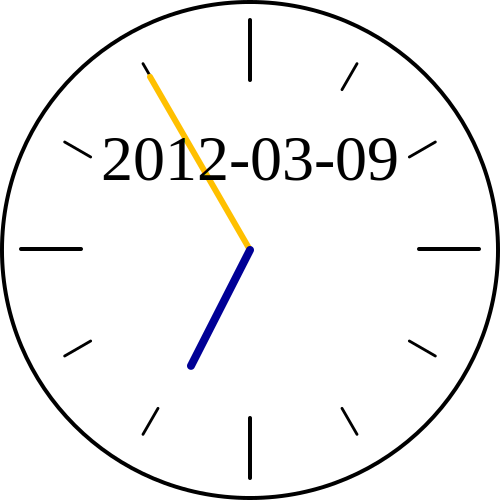
\includegraphics[scale=.4]{get_utc_time.pdf}
  \end{center}
\end{frame}

\begin{frame}

  \begin{center}
  \LARGE
    It's also easy to implement declarative

    \bigskip

    restrictions on your input data.
  \end{center}

\end{frame}

\begin{frame}[fragile]
  \begin{tabular}{l}
  \LARGE So instead of doing this:
  \end{tabular}

  \bigskip

  \begin{lstlisting}
def get_name_of_month(month):
    """Takes an integer between 1-12 and
    returns the name of month as string
    """

    value = int(month)

    if not (1 <= value <= 12):
        raise ValueError(value)

    return datetime(2000,month,1).strftime("%B")
  \end{lstlisting}
\end{frame}

\begin{frame}[fragile]
  \begin{tabular}{l}
  \LARGE You can do this:
  \end{tabular}

  \bigskip

  \begin{lstlisting}[emph={Integer,le,ge}]
class NameOfMonthService(Service):
  @srpc(Integer(ge=1,le=12), _returns=Unicode)
  def get_name_of_month(month):
    return datetime(2000,month,1).strftime("%B")
  \end{lstlisting}
\end{frame}


\begin{frame}[fragile]
  \begin{tabular}{l}
  \LARGE And if you enable validation;
  \end{tabular}

  \bigskip

  \begin{lstlisting}[emph=validator]
from spyne.application import Application
from spyne.protocol.http import HttpRpc

rest = Application([NameOfMonthService],
        tns='spyne.examples.multiprot',
        in_protocol=HttpRpc(validator='soft'),
        out_protocol=HttpRpc()
    )
  \end{lstlisting}

\end{frame}
\begin{frame}[fragile]

  \begin{lstlisting}[language=sh]
$ curl localhost:9912/get_name_of_month?month=3
March
  \end{lstlisting}

\pause
\bigskip

  \begin{lstlisting}[language=sh,basicstyle=\small]
$ curl -D - localhost:9912/get_name_of_month?month=13
HTTP/1.0 400 Bad Request
Date: Sat, 10 Mar 2012 14:21:36 GMT
Server: WSGIServer/0.1 Python/2.7.2
Content-Length: 63
Content-Type: text/plain

Client.ValidationError

The string '13' could not be validated
  \end{lstlisting}

\end{frame}



\begin{frame}
  \huge
  \textbf{So, what's missing?}
  \begin{center}
\Large
  \begin{tabular}{ll}
    \textbf{Protocols}:  & JSON! ProtoBuf! XmlRpc! Thrift! \\
                         & YAML! HTML! (The whole document) \\
    \textbf{Transports}: & SMTP! Files! SPDY! WebSockets!
  \end{tabular}

  \bigskip

  \large
  $\left(
    \begin{tabular}{c}
    and many other things! see the ROADMAP.rst \\
    in the source repo.
  \end{tabular}
  \right)$

  \end{center}
\end{frame}

\begin{frame}
  \frametitle{Additional Information:}

  \begin{center}
  \huge

  \href{http://github.com/arskom/spyne}{github.com/arskom/spyne}

  \bigskip

  \large

  This example and the presentation are in:
  \href{https://github.com/arskom/spyne/tree/master/examples/multiple_protocols}{examples/multiple\_protocols}

  \href{https://github.com/arskom/spyne/tree/master/examples/validation.py}{examples/validation.py}

  \bigskip

  Stay for the sprints! I'll be around!

  \end{center}

\end{frame}

\end{document}
